\section{Regelkreise aus LTI-Systemen}{105}

\subsection{Steuerung} 
    
    \begin{minipage}[c]{0.48\columnwidth}
        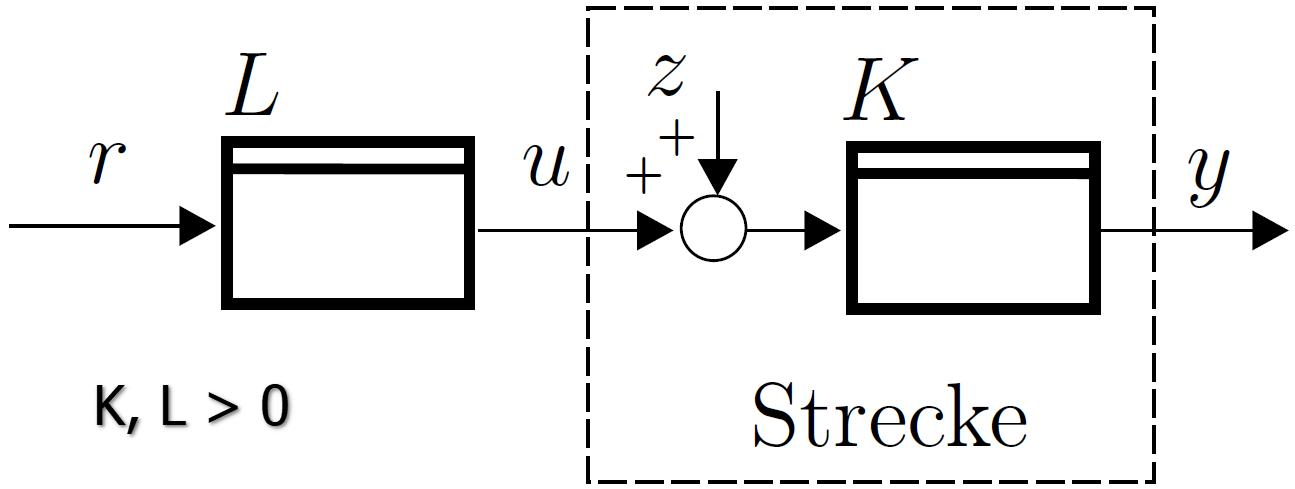
\includegraphics[align=center, width=\columnwidth]{images/steuerung.jpg}
    \end{minipage}
    \hfill
    \begin{minipage}[c]{0.5\columnwidth}
        Eine Steuerung besitzt \textbf{keine Rückkopplung} und ist somit ein \textbf{offener Regelkreis}
        $$ y = \underbrace{K L \cdot r}_{\text{Sensitivität}} + \underbrace{K \cdot z}_{\text{Störung}}$$
    \end{minipage}


\subsection{Regelung}

    \begin{minipage}[c]{0.48\columnwidth}
        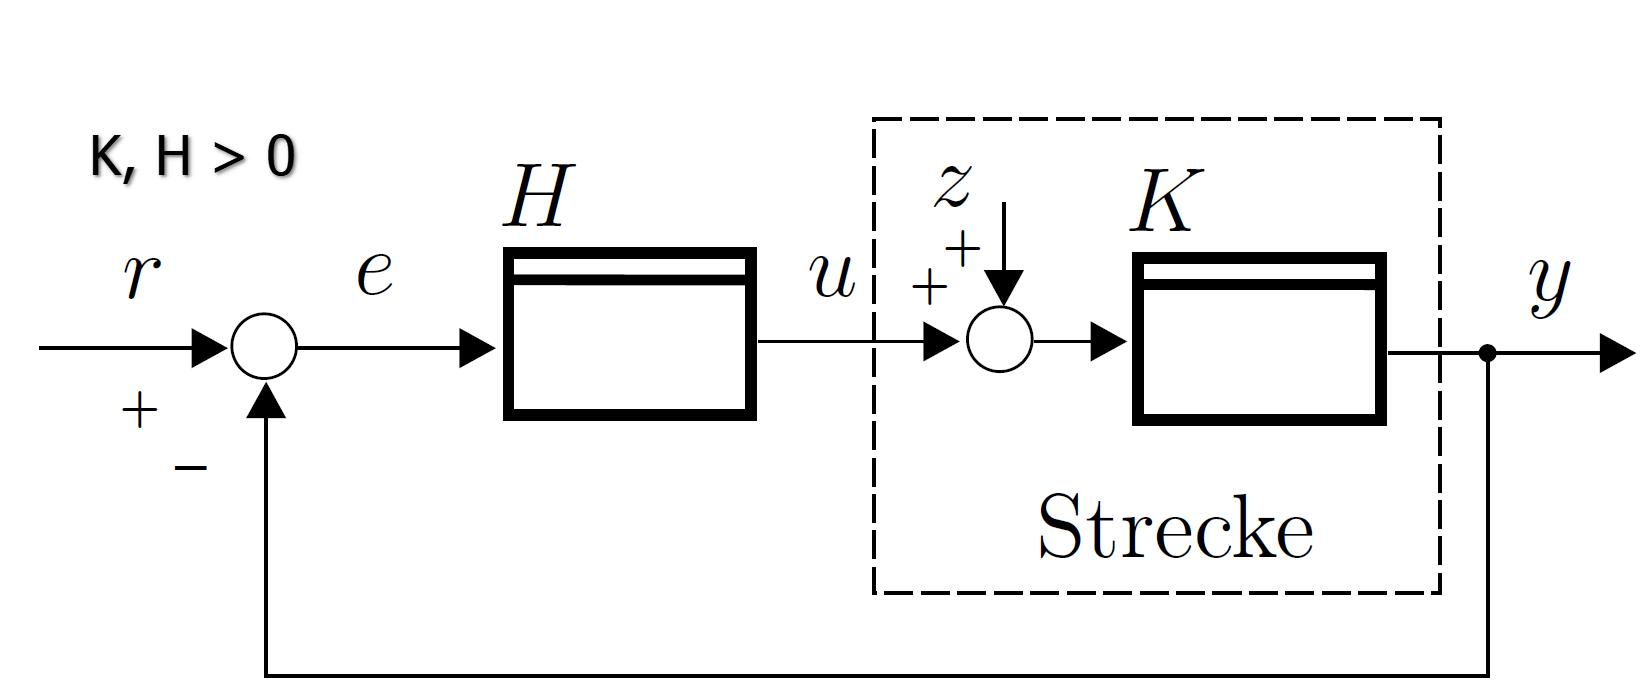
\includegraphics[align=center, width=\columnwidth]{images/regelung.jpg}
    \end{minipage}
    \hfill
    \begin{minipage}[c]{0.5\columnwidth}
        Eine Regelung besitzt eine \textbf{Gegenkopplung}
        $$ y = K H \cdot (r - y) + K \cdot z$$
        $$ y = \underbrace{\frac{K H}{1 + K H} \cdot r}_{\text{Sensitivität}} + \underbrace{\frac{K}{1 + K H} \cdot z}_{\text{Störungsunterdrückung}} $$
    \end{minipage}


\subsubsection{Störungsunterdrückung}{106}

    Ein Regler ist vorteilhaft, um Störungen zu unterdrücken, denn für die Verstärkung $H$ der Störung $z$ gilt:
    $$ \lim\limits_{H \to \infty} \frac{K}{1 + K H} \cdot z = 0 $$
    \textrightarrow\ Hat der Regler eine grosse Verstärkung $H$, so wird die Störung $z$ unterdrückt\\
    \textrightarrow\ Bei einer Steuerung wird die Störung $z$ nicht unterdrückt


\subsubsection{Sensitivität (Empfindlichkeit)}{106}

    Für die Sensitivität eines Reglers gilt:
    $$ \lim\limits_{H \to \infty} \frac{K H}{1 + K H} \cdot r = 1 $$
    \textrightarrow\ Hat der Regler eine grosse Verstärkung $H$, so ist $y \approx r$ (Ausgang $\approx$ Sollwert)\\
    \textrightarrow\ Bei einer Steuerung muss $H = \frac{1}{L}$ sein, damit $y \approx r$


\subsubsection{Stabilitätsproblem}{109-110}

    Sobald ein offener Regelkreis (Steuerung) geschlossen wird, muss darauf geachtet werden, dass das System stabil ist.
    

\subsection{Stabilität eines Systems mit Rückkopplung}

    \begin{tabular}{lll}
        (asymp.) stabil     & Verstärkung $|V| < 1$ & System schwingt nicht \\
        grenzstabil         & Verstärkung $V = -1$  & System schwingt mit konstanter Ampl.\\
        instabil            & Verstärkung $|V| > 1$ & System schwingt mit zunehmender Ampl. 
    \end{tabular}


\subsubsection{Berechnung Grenzstabilität}{111}

    Für Grenzstabilität muss für die Verstärkung des Systems gelten: $V = -1$ 


    \example{Grenzstabilität System aus I-Glied und Totzeitglied}

    \begin{center}
        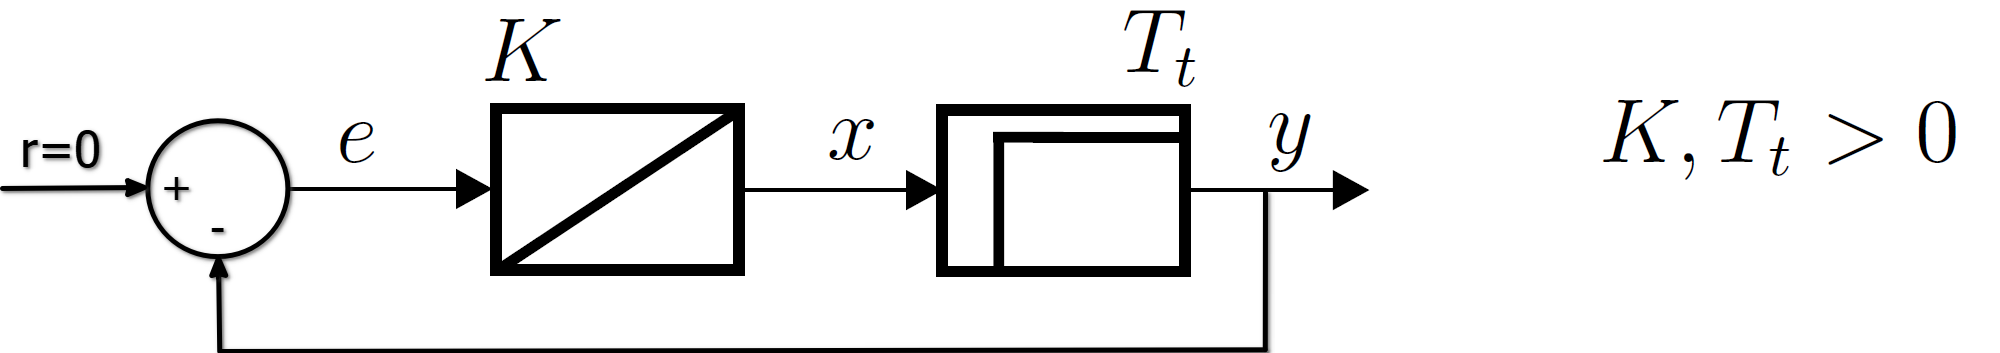
\includegraphics[align=center, width=0.75\columnwidth]{images/gegengekoppeltes_system.png}
    \end{center}

    Es muss gelten: $y(t) = -e(t)$ unter der Annahme, dass $e(t) = A \cdot \cos(\omega t)$

    \vspace*{-0.3cm}        % reduce space before align environment

    \begin{align*}
        x(t) &= K \cdot \int\limits_0^t e(\tau) \diff \tau + x_0 
            = K \cdot \int\limits_0^t A \cdot \cos(\omega \tau) \diff \tau + x_0
            = K \frac{A}{\omega} \sin(\omega \tau) \Big|_0^t + x_0 \\
            &= \frac{K A}{\omega} \sin(\omega t) + \underbrace{x_0}_{0} \\
        y(t) &= x(t - T_t) = \frac{K A}{\omega} \sin(\omega (t - T_t)) = \frac{K A}{\omega} \cos \big( \omega( t- T_t) - \frac{\pi}{2}  \big)
    \end{align*}

 

    $$ \text{Koeffizientenvergleich: } \underbrace{ \cbl{ \frac{K A}{\omega}} \cos \big( \omega t \cor{- \omega T_t - \frac{\pi}{2}}  \big) }_{y(t)}
         = - A \cos(\omega t) = \underbrace{ \cbl{A} \cdot \cos(\omega t \cor{- \pi}) }_{-e(t)} $$
    
    $$ \text{Der Koeffizientenvergleich liefert: } \cbl{\omega = K} \quad \text{und} \quad \cor{\omega = K = \frac{\pi}{2 \cdot T}} $$

    \textrightarrow\ Wenn der Regler die Verstärkung $K$ hat ist das System grenzstabil 
    und das System schwingt für alle Zeit mit der Frequenz $\omega$\\
    \textrightarrow\ Die Verstärkung $K$ muss vermieden werden!

    